\documentclass[11pt]{article}

\usepackage[margin=1in]{geometry}
\usepackage{parskip}
\usepackage{enumitem}
\usepackage{booktabs}
\usepackage{tcolorbox}
\usepackage{hyperref}
\usepackage{titlesec}
\usepackage{xcolor}
\usepackage{longtable}
\usepackage{array}
\usepackage{tikz}
\usetikzlibrary{positioning, arrows.meta, fit, backgrounds, shapes.geometric}

\hypersetup{
    colorlinks=true,
    linkcolor=blue!60!black,
    urlcolor=blue!60!black,
    citecolor=blue!60!black
}

\titleformat{\section}{\Large\bfseries\color{blue!40!black}}{\thesection}{1em}{}
\titleformat{\subsection}{\large\bfseries}{\thesubsection}{1em}{}

\title{\textbf{Two Parallelisms in One Weekend\\
A Workflow Paper for the Darwin Self-Improving Chess Engine}}
\author{Point72 Hackathon \\ \textit{Supplement to the Darwin proposal}}
\date{}

\begin{document}
\maketitle

\hrule
\vspace{0.6em}

\begin{abstract}
\noindent Darwin is a self-improving chess engine: each generation, a
strategist proposes improvements to the reigning champion, parallel
builders implement them, a validator gates the candidates, a round-robin
tournament plays them, and the top two engines advance. It was built in
a weekend hackathon by five engineers, each driving a separate AI coding
agent against a small set of frozen contracts. This paper documents the
\emph{workflow} rather than the engine: the two parallelisms
(engine-time and build-time) that the project was structured around, the
three contracts that decoupled the workstreams, the per-engineer scopes,
the merge sequence that glued it together, and what worked and didn't
when the same dual-parallelism shape was applied to humans, agents, and
runtime processes simultaneously.
\end{abstract}

\hrule
\vspace{0.4em}

\tableofcontents
\vspace{0.6em}
\hrule

\section{The Two Parallelisms}
\label{sec:two-parallelisms}

The shape of Darwin is the same shape twice. At runtime, one strategist
fans out work to several builders that run in parallel. At build time,
five engineers each drove a separate AI coding agent against the same
codebase, in parallel, on five branches. We call these \emph{engine-time
parallelism} and \emph{build-time parallelism}, and the rest of this
paper is organised around the observation that they share the same
critical-path ingredient: a small set of frozen interfaces that let
independent producers and consumers proceed without waiting on each
other.

\textbf{Engine-time parallelism} (Figure~\ref{fig:runtime-pipeline}) is
the runtime loop. The reigning champion is shown to a strategist agent;
the strategist returns a fixed-shape set of improvement
\emph{questions}, each tagged with one of the categories
\texttt{search}, \texttt{evaluation}, \texttt{book}, \texttt{sampling},
\texttt{prompt}. \emph{N} builder agents run concurrently, one per
question, each producing a Python module that satisfies the
\texttt{Engine} Protocol. A validator runs cheap static gates and a
smoke game against \texttt{RandomEngine} to drop crashers and
no-op fallbacks. The surviving candidates plus the previous-generation
incumbents play a round-robin (both colours per pairing,
\texttt{games\_per\_pairing} configurable). Selection ranks by
tournament score with random tiebreak; the top two engines seed the
next generation.

\begin{figure}[h!]
\centering
% fig-runtime-pipeline.tex
% Engine-time parallelism: strategist -> N parallel builders -> validator
% -> round-robin -> top-2 selection. Inputs: only TikZ libraries listed
% in workflow.tex's preamble.
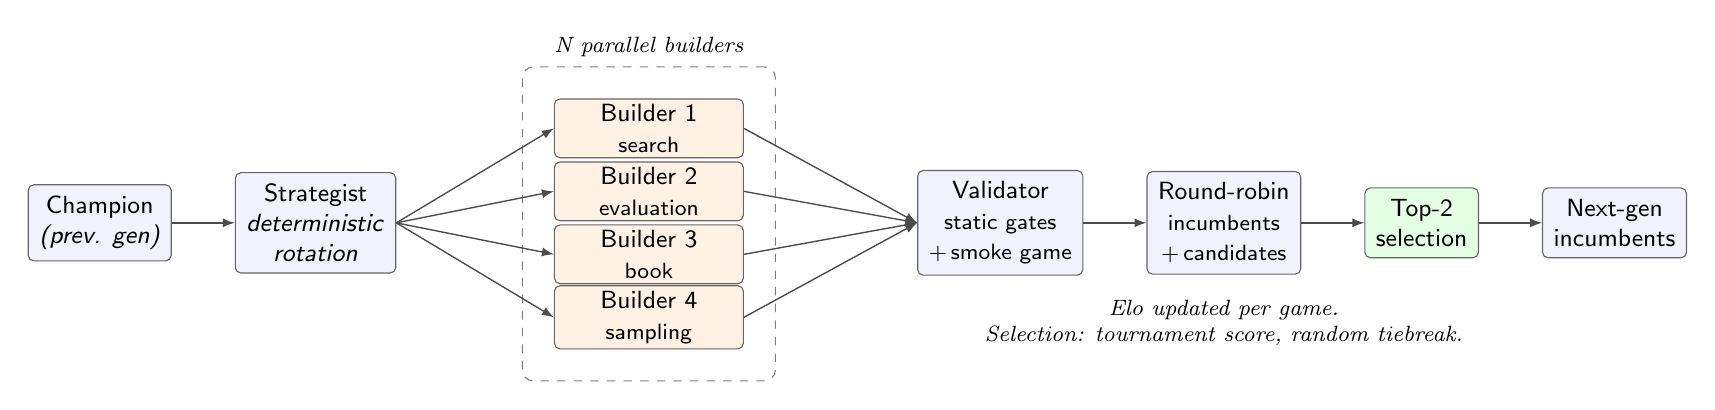
\begin{tikzpicture}[
    font=\small\sffamily,
    node distance=6mm and 8mm,
    box/.style={
        draw=black!60, rounded corners=2pt, fill=blue!5,
        minimum height=8mm, align=center, inner sep=4pt,
    },
    builder/.style={
        draw=black!60, rounded corners=2pt, fill=orange!10,
        minimum width=24mm, minimum height=7mm, align=center, inner sep=2pt,
    },
    sel/.style={
        draw=black!60, rounded corners=2pt, fill=green!10,
        minimum height=8mm, align=center, inner sep=4pt,
    },
    arrow/.style={-latex, draw=black!70, line width=0.5pt},
    pile/.style={draw=black!50, dashed, rounded corners=4pt, inner sep=4mm},
]

\node[box] (champ) {Champion\\\textit{(prev. gen)}};
\node[box, right=of champ] (strat) {Strategist\\\textit{deterministic}\\\textit{rotation}};

\node[builder, right=20mm of strat, yshift=12mm] (b1) {Builder 1\\\footnotesize search};
\node[builder, right=20mm of strat, yshift=4mm]  (b2) {Builder 2\\\footnotesize evaluation};
\node[builder, right=20mm of strat, yshift=-4mm] (b3) {Builder 3\\\footnotesize book};
\node[builder, right=20mm of strat, yshift=-12mm](b4) {Builder 4\\\footnotesize sampling};

\node[box, right=22mm of b2, yshift=-4mm] (val) {Validator\\\footnotesize static gates\\\footnotesize +\,smoke game};
\node[box, right=of val] (rr) {Round-robin\\\footnotesize incumbents\\\footnotesize +\,candidates};
\node[sel, right=of rr] (top) {Top-2\\selection};
\node[box, right=of top] (next) {Next-gen\\incumbents};

\draw[arrow] (champ) -- (strat);
\draw[arrow] (strat.east) -- (b1.west);
\draw[arrow] (strat.east) -- (b2.west);
\draw[arrow] (strat.east) -- (b3.west);
\draw[arrow] (strat.east) -- (b4.west);
\draw[arrow] (b1.east) -- (val.west);
\draw[arrow] (b2.east) -- (val.west);
\draw[arrow] (b3.east) -- (val.west);
\draw[arrow] (b4.east) -- (val.west);
\draw[arrow] (val) -- (rr);
\draw[arrow] (rr) -- (top);
\draw[arrow] (top) -- (next);

\begin{pgfonlayer}{background}
\node[pile, fit=(b1)(b2)(b3)(b4), label={[font=\footnotesize\itshape]above:N parallel builders}] {};
\end{pgfonlayer}

\node[font=\footnotesize\itshape, below=2mm of rr, align=center]
    {Elo updated per game.\\Selection: tournament score, random tiebreak.};

\end{tikzpicture}

\caption{Engine-time parallelism: one strategist fans out to N parallel
builders; the validator gates them; the round-robin scores the cohort;
the top-2 engines seed the next generation. Source:
\href{run:../backend/darwin/orchestration/generation.py}{\texttt{backend/darwin/orchestration/generation.py}}.}
\label{fig:runtime-pipeline}
\end{figure}

\textbf{Build-time parallelism} (Figure~\ref{fig:build-parallelism}) is
the human and agent process. Five engineers (Persons A through E),
each paired with their own AI coding agent, opened five branches and
shipped five workstreams in parallel. The first hour was spent
\emph{not} writing code: it was spent agreeing on the three contracts
described in \S\ref{sec:frozen-contracts}. Once those were frozen, each
engineer wrote against fakes for the other four workstreams, and only
integrated when their own piece was real.

\begin{figure}[h!]
\centering
% fig-build-parallelism.tex
% Build-time parallelism: 5 engineers + 5 agents on 5 branches against
% frozen contracts. Gantt-style timeline with merge points.
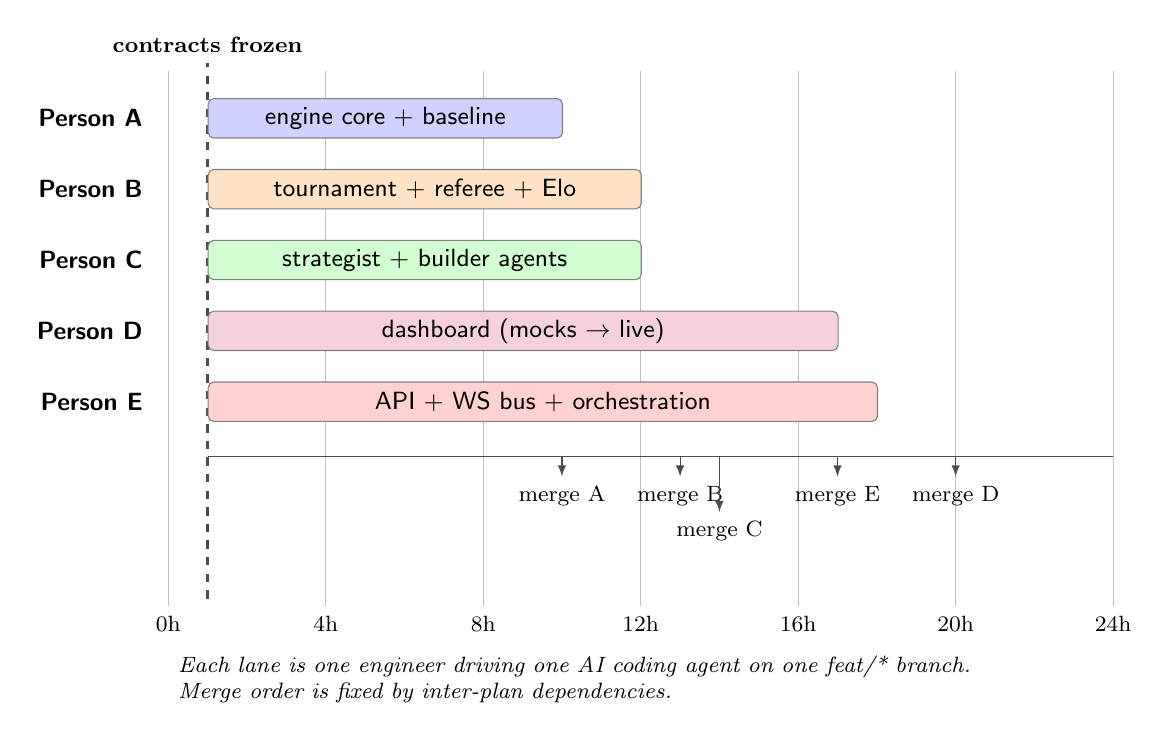
\begin{tikzpicture}[
    font=\small\sffamily,
    bar/.style={draw=black!50, rounded corners=2pt, minimum height=5mm, inner sep=2pt},
    a/.style={bar, fill=blue!18},
    b/.style={bar, fill=orange!22},
    c/.style={bar, fill=green!18},
    d/.style={bar, fill=purple!18},
    e/.style={bar, fill=red!18},
    freeze/.style={draw=black!70, very thick, dashed},
    merge/.style={draw=black!70, line width=0.4pt},
    tick/.style={font=\footnotesize, anchor=north},
]

\def\xscale{0.5}

% Hour grid
\foreach \h in {0,4,8,12,16,20,24} {
    \draw[gray!50] (\h*\xscale, -1.2) -- (\h*\xscale, 5.6);
    \node[tick] at (\h*\xscale, -1.2) {\h h};
}

% Hour-0 contract freeze
\draw[freeze] (1*\xscale, -1.1) -- (1*\xscale, 5.7)
    node[above, font=\footnotesize\bfseries] {contracts frozen};

% Workstream lanes
\node[anchor=east] at (-0.2, 5.0) {\bfseries Person A};
\node[a, anchor=west, minimum width={9*\xscale*1cm}]  at (1*\xscale, 5.0) {engine core + baseline};

\node[anchor=east] at (-0.2, 4.1) {\bfseries Person B};
\node[b, anchor=west, minimum width={11*\xscale*1cm}] at (1*\xscale, 4.1) {tournament + referee + Elo};

\node[anchor=east] at (-0.2, 3.2) {\bfseries Person C};
\node[c, anchor=west, minimum width={11*\xscale*1cm}] at (1*\xscale, 3.2) {strategist + builder agents};

\node[anchor=east] at (-0.2, 2.3) {\bfseries Person D};
\node[d, anchor=west, minimum width={16*\xscale*1cm}] at (1*\xscale, 2.3) {dashboard (mocks $\to$ live)};

\node[anchor=east] at (-0.2, 1.4) {\bfseries Person E};
\node[e, anchor=west, minimum width={17*\xscale*1cm}] at (1*\xscale, 1.4) {API + WS bus + orchestration};

% Merge axis
\draw[merge] (1*\xscale, 0.7) -- (24*\xscale, 0.7);

% Merge labels — staggered vertically so 13h/14h labels don't collide
\foreach \xh/\lbl/\dy in {10/A/0, 13/B/0, 14/C/-0.45, 17/E/0, 20/D/0} {
    \draw[merge, -latex] (\xh*\xscale, 0.7) -- (\xh*\xscale, 0.45 + \dy);
    \node[font=\footnotesize, anchor=north] at (\xh*\xscale, 0.45 + \dy) {merge \lbl};
}

% Bottom caption — width-constrained so it fits on the page
\node[font=\footnotesize\itshape, anchor=north west, align=left,
      text width={24*\xscale*1cm}]
    at (0, -1.7)
    {Each lane is one engineer driving one AI coding agent on one feat/* branch.\\
     Merge order is fixed by inter-plan dependencies.};

\end{tikzpicture}

\caption{Build-time parallelism: five engineer/agent pairs working
against frozen contracts on parallel \texttt{feat/*} branches over a
24-hour build window. Merge order is fixed by inter-plan dependencies.}
\label{fig:build-parallelism}
\end{figure}

The two parallelisms are not analogies. They are the same engineering
move in two domains: \emph{commit to a small set of interfaces, then let
producers and consumers run concurrently against them.} The runtime
loop uses asyncio; the build process uses git branches. The contracts
are different files, but the discipline is the same.

\section{Frozen Contracts as Parallelization Seams}
\label{sec:frozen-contracts}

Three files were declared frozen at hour 1 and not modified again
without team sync. Each one cleanly decoupled a producer from a
consumer; together they were enough to let the five workstreams ship in
parallel. Figure~\ref{fig:frozen-contracts} summarises them.

\begin{figure}[h!]
\centering
% fig-frozen-contracts.tex
% Three frozen contracts as parallelization seams. Each pillar shows the
% interface, the producers, and the consumers it decouples.
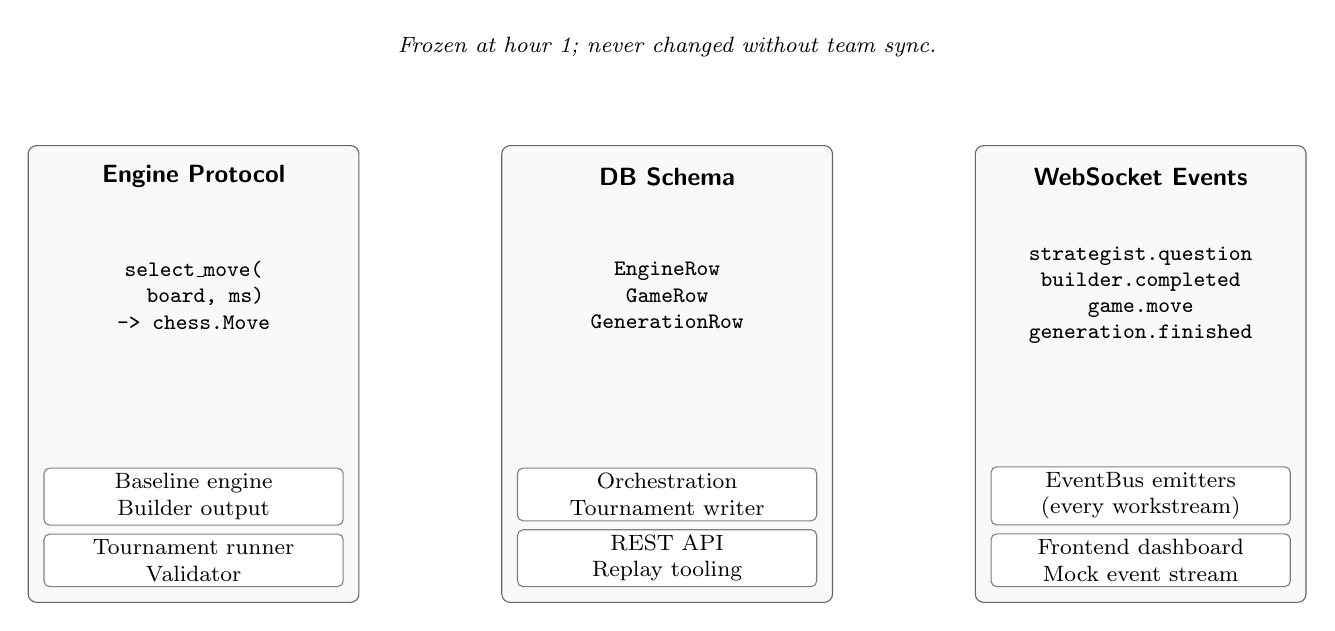
\begin{tikzpicture}[
    font=\small\sffamily,
    pillar/.style={
        draw=black!60, rounded corners=3pt, fill=gray!5,
        minimum width=42mm, minimum height=58mm, align=center, inner sep=4pt,
    },
    head/.style={font=\bfseries\sffamily\small, align=center},
    code/.style={font=\ttfamily\footnotesize, align=center},
    side/.style={
        draw=black!50, rounded corners=2pt, fill=white,
        minimum width=38mm, align=center, inner sep=2pt, font=\footnotesize,
    },
    arrow/.style={-latex, draw=black!70, line width=0.4pt},
]

% --- pillar 1: Engine Protocol ---
\node[pillar] (p1) at (0,0) {};
\node[head] at (p1.north) [yshift=-4mm] {Engine Protocol};
\node[code] at (p1.center) [yshift=10mm]
    {\texttt{select\_move(}\\\texttt{~~board, ms)}\\\texttt{-> chess.Move}};
\node[side, above=2mm of p1.south] (p1c) {Tournament runner\\Validator};
\node[side, above=1mm of p1c] (p1p) {Baseline engine\\Builder output};

% --- pillar 2: DB schema ---
\node[pillar, right=18mm of p1] (p2) {};
\node[head] at (p2.north) [yshift=-4mm] {DB Schema};
\node[code] at (p2.center) [yshift=10mm]
    {\texttt{EngineRow}\\\texttt{GameRow}\\\texttt{GenerationRow}};
\node[side, above=2mm of p2.south] (p2c) {REST API\\Replay tooling};
\node[side, above=1mm of p2c] (p2p) {Orchestration\\Tournament writer};

% --- pillar 3: WS events ---
\node[pillar, right=18mm of p2] (p3) {};
\node[head] at (p3.north) [yshift=-4mm] {WebSocket Events};
\node[code] at (p3.center) [yshift=10mm]
    {\texttt{strategist.question}\\\texttt{builder.completed}\\\texttt{game.move}\\\texttt{generation.finished}};
\node[side, above=2mm of p3.south] (p3c) {Frontend dashboard\\Mock event stream};
\node[side, above=1mm of p3c] (p3p) {EventBus emitters\\(every workstream)};

% top label across
\node[font=\footnotesize\itshape, above=10mm of p2.north]
    {Frozen at hour 1; never changed without team sync.};

\end{tikzpicture}

\caption{The three frozen contracts and what each decouples.
The Engine Protocol decouples engine producers from the tournament
runner. The DB schema decouples the orchestrator from the API. The
WebSocket events decouple the backend from the frontend.}
\label{fig:frozen-contracts}
\end{figure}

\subsection{Engine Protocol}
\href{run:../backend/darwin/engines/base.py}{\texttt{backend/darwin/engines/base.py}}.
A \texttt{runtime\_checkable} \texttt{Protocol} with three attributes
(\texttt{name}, \texttt{generation}, \texttt{lineage}) and one async
method, \texttt{select\_move(board, time\_remaining\_ms) -> chess.Move}.
This is the seam that lets a builder agent emit a Python module at
runtime that drops into the same tournament runner as the hand-written
baseline. It also lets Person B (tournament) write tests against
\texttt{RandomEngine} on day one, before Person A's
\texttt{BaselineEngine} existed, and before any builder-generated
engine had been produced. The Protocol's smallness is the point: the
fewer fields, the fewer ways the contract can drift.

\subsection{DB Schema}
\href{run:../backend/darwin/storage/models.py}{\texttt{backend/darwin/storage/models.py}}.
Three SQLModel tables: \texttt{EngineRow}, \texttt{GameRow},
\texttt{GenerationRow}. The orchestrator writes to all three; the
REST API reads from all three; the replay tool reads from the first two
and re-emits WebSocket events. Freezing this schema let Person D's
frontend mock generation traces against fake JSON, and let Person B's
tournament runner write game records before Person E's API existed to
read them.

\subsection{WebSocket Events}
\href{run:../backend/darwin/api/websocket.py}{\texttt{backend/darwin/api/websocket.py}}
on the backend, mirrored in
\href{run:../frontend/src/api/events.ts}{\texttt{frontend/src/api/events.ts}}
on the frontend. A discriminated union over event types
(\texttt{generation.started}, \texttt{strategist.question},
\texttt{builder.completed}, \texttt{game.move}, \texttt{game.finished},
\texttt{generation.finished}, plus cancellation and state-clear events
added in follow-ups). Both files are FROZEN comments at the top; the
two must stay aligned, and any change requires a paired edit. This is
the contract that let Person D ship a fully working dashboard
\emph{against a hand-written mock event stream} for most of the
hackathon, then flip a query-string flag when Person E's bus came up.

The pattern across all three contracts: \emph{shape committed early,
both sides mock against it, real implementations land at their own
pace.} The cost of disagreement was paid once, at hour 1, instead of
recurring at every integration.

\section{Per-Engineer Workstreams (A--E)}
\label{sec:workstreams}

The five workstreams below each owned one directory tree and one
\texttt{feat/*} branch. Plan documents in
\href{run:../plans/}{\texttt{plans/}} define the scopes; this section
abstracts them into a half-page each.

\subsection{Person A --- Engine Core \& Baseline}
Branch \texttt{feat/engine-core}; plan
\href{run:../plans/person-a-engine-core.md}{\texttt{plans/person-a-engine-core.md}}.
Owns the \texttt{Engine} Protocol, the
\texttt{BaseLLMEngine} convenience class, the generation-0
\texttt{BaselineEngine}, the \texttt{RandomEngine} sparring partner,
and the \texttt{registry.load\_engine} dynamic loader. \emph{Critical
property:} every other workstream depends on this Protocol, so
shipping a frozen \texttt{base.py} with a stub baseline early was the
unblocker for the whole project. Tests at this level are tight: a
single legal-move assertion for the baseline plus four registry tests
covering both dotted-module and filesystem-path loads.

\subsection{Person B --- Tournament \& Referee}
Branch \texttt{feat/tournament}; plan
\href{run:../plans/person-b-tournament.md}{\texttt{plans/person-b-tournament.md}}.
Owns \texttt{play\_game} (one game with per-move time control and
graceful loss adjudication), \texttt{round\_robin} (parallel pairing
schedule via \texttt{asyncio.gather}, capped by a semaphore added in
follow-up~1), the Elo update (\texttt{K=32}), and the
\texttt{select\_top\_n} anti-regression gate. The whole pipeline's
runtime budget --- whether 3 generations can finish in a hackathon ---
lives or dies on this module's parallelism, which is why Person B was
also responsible for the \texttt{eval\_match.py} headline-number CLI.

\subsection{Person C --- Strategist + Builder Agents}
Branch \texttt{feat/agents}; plan
\href{run:../plans/person-c-agents.md}{\texttt{plans/person-c-agents.md}}.
Owns \texttt{propose\_questions} (the strategist) and
\texttt{build\_engine}/\texttt{validate\_engine} (the builder). The
strategist returns 2--4 distinct improvement questions, one per
category; the builder calls a \texttt{submit\_engine} tool whose
\texttt{input\_schema} forces a single-string \texttt{code} field. The
validator runs static gates (forbidden-import regex, required-pattern
regex, \texttt{ast.parse}) and a smoke game against
\texttt{RandomEngine}. Person C's stub implementations were the single
most important early ship: they let Person E wire the orchestrator
end-to-end against fakes hours before the real agents were ready.

\subsection{Person D --- Frontend Dashboard}
Branch \texttt{feat/frontend}; plan
\href{run:../plans/person-d-frontend.md}{\texttt{plans/person-d-frontend.md}}.
Owns the React + Vite + Tailwind dashboard, including
\texttt{LiveBoard}, \texttt{EloChart}, \texttt{StrategistFeed},
\texttt{Bracket}, and \texttt{GenerationTimeline}. Built against
\texttt{src/hooks/mockEvents.ts} for offline development and switched
to the live WebSocket via a \texttt{?mock=1} query-string flag once
Person E shipped the bus. The flag was the entire integration: the
event shapes were guaranteed by the contract.

\subsection{Person E --- Infra, API, Orchestration, Demo}
Branch \texttt{feat/infra}; plan
\href{run:../plans/person-e-infra.md}{\texttt{plans/person-e-infra.md}}.
Owns the integrator's pile: the SQLite database, the FastAPI server,
the WebSocket bus, the top-level
\texttt{orchestration/generation.py} loop that calls into A, B, and
C, the shared LLM helper with semaphore + retry, the Procfile, the
seed and replay scripts, and the demo plan. Person E is the only role
that touches every other workstream; the corresponding mitigation is
that they touch \emph{only} through the three frozen contracts.

\section{The Runtime Agent Pipeline}
\label{sec:pipeline}

The orchestration loop in
\href{run:../backend/darwin/orchestration/generation.py}{\texttt{generation.py}}
is the engine-time parallelism made concrete. One generation, in
order:

\begin{enumerate}[leftmargin=*]
\item \textbf{Pool warm-up.} \texttt{warm\_modal\_pool(40)} kicks off
40 Modal containers in the background while the strategist and
builders run. This is a small but important asynchrony: the
\(\sim\)25--30 seconds spent on agent calls is enough for the warm
pool to be ready by the time the tournament dispatches.
\item \textbf{Strategist.}
\texttt{propose\_questions(champion\_src, history)} returns a list of
\texttt{Question} objects, each with a category and a free-text
hypothesis. Reads the champion's source via \texttt{inspect.getsource}
so the agent prompts are grounded in the actual code under
modification, not an abstract description.
\item \textbf{Parallel builders.}
\texttt{asyncio.gather(*[build\_engine(...) for q in questions])}.
Each builder calls the builder LLM with the
\texttt{submit\_engine} tool, runs the static gates, and writes
\texttt{engines/generated/<name>.py}.
\item \textbf{Validator.} Each candidate is loaded through the
registry and plays one short game against \texttt{RandomEngine}.
Crashers, illegal-move emitters, and time-outers are dropped before
they reach the tournament. The
\texttt{builder.completed} WebSocket event fires the moment each
candidate's verdict is known, so the dashboard sees results stream in
rather than batched at the end.
\item \textbf{Round-robin.}
\texttt{round\_robin(cohort, games\_per\_pairing, time\_per\_move\_ms,
on\_event=bus.emit)}. The cohort is incumbents \(\cup\) accepted
candidates --- typically 4--6 engines, so 60--90 games. The
\texttt{max\_parallel\_games} semaphore caps actual concurrency to
keep the LLM provider's quota in line.
\item \textbf{Elo update.}
\texttt{update\_ratings\_for\_games(ratings, standings.games)} applies
\texttt{K=32} per game. New candidates seed at 1500.
\item \textbf{Selection.} \texttt{select\_top\_n} ranks by tournament
score with random tiebreak; the primary incumbent is the
anti-regression baseline.
\item \textbf{Persist + emit.} A \texttt{GenerationRow} with the
strategist questions, a \texttt{GameRow} per game, an
\texttt{EngineRow} per accepted candidate, and a final
\texttt{generation.finished} event with the post-tournament Elo for
every cohort member.
\end{enumerate}

The whole-system architecture, including how this loop hangs off the
API, the database, and the optional Modal backend, is shown in
Figure~\ref{fig:meta-architecture}.

\begin{figure}[h!]
\centering
% fig-meta-architecture.tex
% Whole-system architecture: backend modules (top-left), storage + event
% bus (bottom band), API surface + frontend (right). Explicit absolute
% coordinates throughout to keep boxes from overlapping.
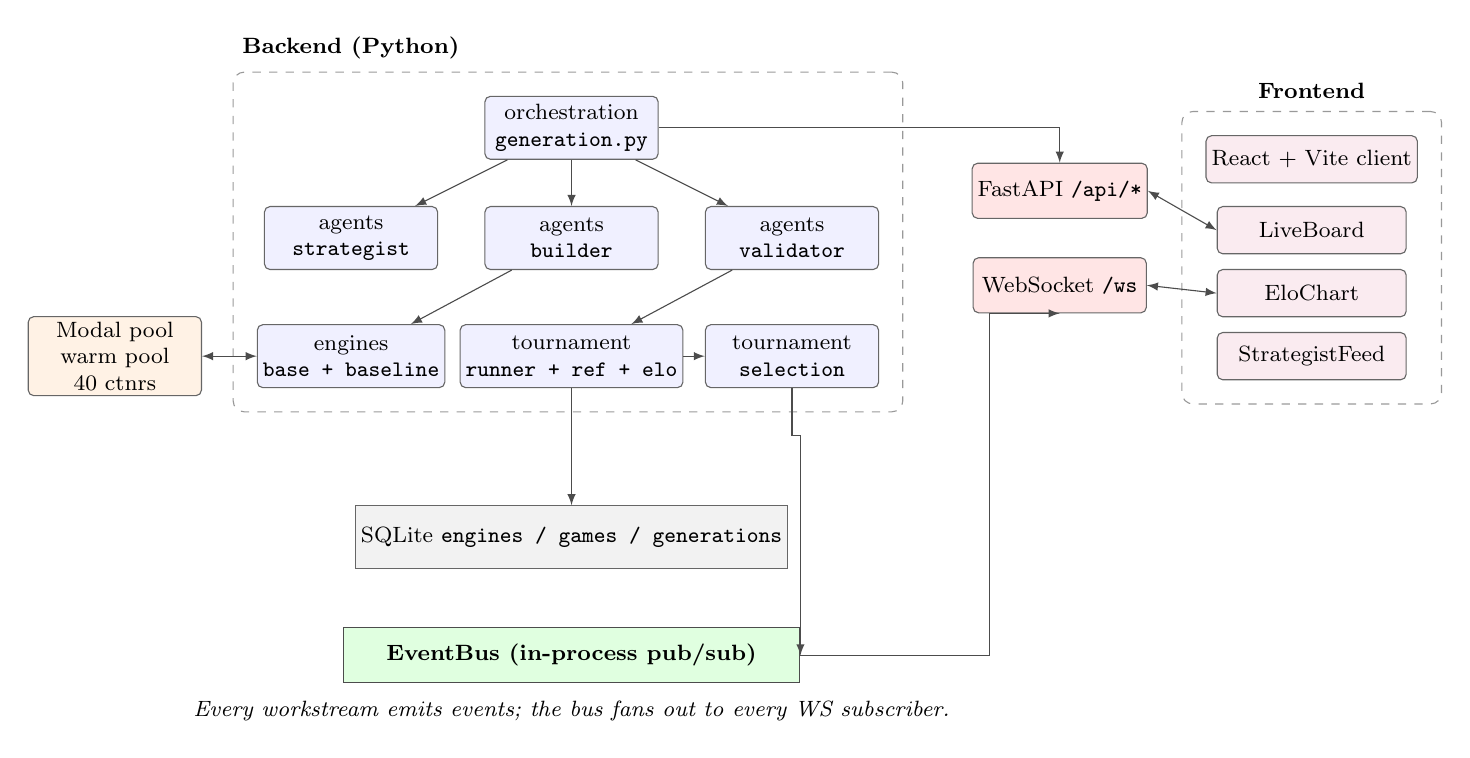
\begin{tikzpicture}[
    font=\small\sffamily,
    x=1cm, y=1cm,
    mod/.style={
        draw=black!60, rounded corners=2pt, fill=blue!6,
        minimum width=22mm, minimum height=8mm, align=center,
        inner sep=2pt, font=\footnotesize,
    },
    api/.style={
        draw=black!60, rounded corners=2pt, fill=red!10,
        minimum width=22mm, minimum height=7mm, align=center,
        inner sep=2pt, font=\footnotesize,
    },
    store/.style={
        draw=black!60, fill=gray!10,
        minimum width=44mm, minimum height=8mm, align=center,
        inner sep=2pt, font=\footnotesize,
    },
    fe/.style={
        draw=black!60, rounded corners=2pt, fill=purple!8,
        minimum width=24mm, minimum height=6mm, align=center,
        inner sep=2pt, font=\footnotesize,
    },
    modal/.style={
        draw=black!60, rounded corners=2pt, fill=orange!10,
        minimum width=22mm, minimum height=10mm, align=center,
        inner sep=2pt, font=\footnotesize,
    },
    bus/.style={
        draw=black!70, fill=green!12,
        minimum width=58mm, minimum height=7mm, align=center,
        inner sep=2pt, font=\footnotesize\bfseries,
    },
    arrow/.style={-latex, draw=black!70, line width=0.4pt},
    biarr/.style={latex-latex, draw=black!70, line width=0.4pt},
    group/.style={
        draw=black!40, dashed, rounded corners=4pt, inner sep=3mm,
    },
]

% ── Backend cluster: agents row + engines/tournament row ─────────────
\node[mod] (orch)   at (1.2, 5.8) {orchestration\\\texttt{generation.py}};
\node[mod] (strat)  at (-1.6, 4.4) {agents\\\texttt{strategist}};
\node[mod] (build)  at (1.2, 4.4)  {agents\\\texttt{builder}};
\node[mod] (val)    at (4.0, 4.4)  {agents\\\texttt{validator}};

\node[mod] (eng)    at (-1.6, 2.9) {engines\\\texttt{base + baseline}};
\node[mod] (tour)   at (1.2, 2.9)  {tournament\\\texttt{runner + ref + elo}};
\node[mod] (sel)    at (4.0, 2.9)  {tournament\\\texttt{selection}};

\begin{pgfonlayer}{background}
\node[group, fit=(orch)(strat)(val)(eng)(sel),
      label={[font=\footnotesize\bfseries, anchor=south west, yshift=1pt]north west:Backend (Python)}] (be) {};
\end{pgfonlayer}

% ── Modal pool (left of backend) ─────────────────────────────────────
\node[modal] (modal) at (-4.6, 2.9) {Modal pool\\\footnotesize warm pool\\\footnotesize 40 ctnrs};

% ── Storage row, well below backend ──────────────────────────────────
\node[store] (db) at (1.2, 0.6) {SQLite \texttt{engines / games / generations}};

% ── Event bus, in its own band below storage ─────────────────────────
\node[bus] (bus) at (1.2, -0.9) {EventBus (in-process pub/sub)};
\node[font=\footnotesize\itshape, below=1mm of bus, align=center]
    {Every workstream emits events; the bus fans out to every WS subscriber.};

% ── API column ───────────────────────────────────────────────────────
\node[api] (api1) at (7.4, 5.0) {FastAPI \texttt{/api/*}};
\node[api] (api2) at (7.4, 3.8) {WebSocket \texttt{/ws}};

% ── Frontend column ──────────────────────────────────────────────────
\node[fe] (cli)   at (10.6, 5.4) {React + Vite client};
\node[fe] (board) at (10.6, 4.5) {LiveBoard};
\node[fe] (chart) at (10.6, 3.7) {EloChart};
\node[fe] (feed)  at (10.6, 2.9) {StrategistFeed};
\begin{pgfonlayer}{background}
\node[group, fit=(cli)(board)(chart)(feed),
      label={[font=\footnotesize\bfseries, anchor=south, yshift=1pt]north:Frontend}] (fe) {};
\end{pgfonlayer}

% ── Edges ────────────────────────────────────────────────────────────
\draw[arrow] (orch) -- (strat);
\draw[arrow] (orch) -- (build);
\draw[arrow] (orch) -- (val);
\draw[arrow] (val)  -- (tour);
\draw[arrow] (tour) -- (sel);
\draw[arrow] (build) -- (eng);

% backend -> SQLite
\draw[arrow] (tour.south) -- (db.north);

% backend -> bus (route around storage)
\draw[arrow] (sel.south) -- ++(0,-0.6) -| (bus.east);

% bus -> WebSocket  (route up the right side, NOT through storage)
\draw[arrow] (bus.east) -- ++(2.4,0) |- (api2.south);

% backend -> API
\draw[arrow] (orch.east) -| (api1.north);

% API <-> frontend
\draw[biarr] (api1.east) -- (board.west);
\draw[biarr] (api2.east) -- (chart.west);

% engines <-> Modal
\draw[biarr] (eng.west) -- (modal.east);

\end{tikzpicture}

\caption{Whole-system architecture: backend modules, SQLite store,
event bus, optional Modal pool for engine execution, FastAPI surface,
React frontend.}
\label{fig:meta-architecture}
\end{figure}

\section{Merge Order and Integration}
\label{sec:merge-order}

Inter-plan dependencies dictated a strict merge order. From
\href{run:../plans/README.md}{\texttt{plans/README.md}}:

\begin{enumerate}[leftmargin=*]
\item \textbf{Person A merges \texttt{feat/engine-core}.} The Protocol
and \texttt{RandomEngine} go live; B and C unblock.
\item \textbf{Person B merges \texttt{feat/tournament}.} The runner
exists in main; E can wire orchestration against real games.
\item \textbf{Person C merges \texttt{feat/agents}.} Real strategist
and builder land; E's orchestration runs end-to-end against real
agents.
\item \textbf{Person E merges \texttt{feat/infra}.} API + WS bus go
live; D switches off mocks.
\item \textbf{Person D merges \texttt{feat/frontend}.} Demo-ready.
\end{enumerate}

The order is not a \emph{decoration}; each merge unblocks the next
one. But because each downstream consumer was already mocking against
the frozen contract, no upstream merge \emph{forced} a downstream
rewrite. A second merge of \texttt{feat/agents} that subtly broke the
\texttt{Question} dataclass would still ripple, but the contract was
designed to make that ripple narrow: the union of fields the
orchestrator reads off a \texttt{Question} is \texttt{index},
\texttt{category}, \texttt{text}.

Four follow-up branches landed after the initial five:
\href{run:../plans/followup-1-tournament-concurrency.md}{tournament
concurrency},
\href{run:../plans/followup-2-builder-quality.md}{builder quality
gate},
\href{run:../plans/followup-3-champion-resume.md}{champion resume},
and
\href{run:../plans/followup-4-frontend-polish.md}{frontend polish}.
Each was scoped to a single workstream's directory tree --- by
construction, since the frozen contracts were already covering the
seams.

\section{What Worked, What Didn't, What We'd Change}
\label{sec:retro}

\subsection{What worked}

\textbf{Hour-1 contract freeze.} Pre-committing the three contracts
made the rest of the day a sequence of independent local optimisations.
None of the workstreams were blocked on inter-team coordination
between hour 2 and hour 16.

\textbf{Mocks before reals.} Person D's mock event stream and
Person C's stub agents both made their dependents productive
\emph{before} the real implementations existed. The pattern was
explicit in every plan: ship a stub, then ship the real.

\textbf{The validator's smoke game.} Catching a builder-generated
engine that times out, returns illegal moves, or crashes on the
opening position --- before it can pollute the tournament --- saved
generations that would otherwise have been pure noise.

\textbf{Per-event streaming on the bus.} The dashboard sees
\texttt{builder.completed} fire as each candidate's verdict resolves,
not in a batch. The loop felt live during demos, not deferred.

\subsection{What didn't}

\textbf{Builder hallucinated import.} Every builder-generated engine
in early generations contained
\texttt{from darwin import config as settings}, which imports the
\emph{module} not the settings instance and then silently raises
\texttt{AttributeError} caught by the engine's own fallback. Net
effect: the engine plays \texttt{next(iter(legal\_moves))} forever,
the validator's smoke game passes, the tournament is meaningless.
Follow-up~2 added the explicit-imports section to the prompt and a
banned-import regex on the validator side. Lesson: \emph{a fallback
that hides bugs is worse than a crash}.

\textbf{Tournament concurrency self-immolation.} A
\texttt{round\_robin} that fires every pairing in parallel will, on a
slow LLM provider, stack moves until the per-move 25\,s timeout
trips on every game and every game terminates on \texttt{time}. The
``winner'' becomes whichever bug fires last. Follow-up~1 added a
\texttt{max\_parallel\_games} semaphore (default 2). Lesson:
\emph{parallelism on top of a rate-limited resource needs to be
gated, not multiplied}.

\textbf{API path didn't resume the lineage.}
\texttt{run\_generation\_task} hard-coded the baseline as the
champion for every API-triggered run. The CLI threaded the champion
forward correctly, but \texttt{POST /api/generations/run} would
restart from baseline-v0 every time, breaking the entire
self-improvement premise. Follow-up~3 loaded the previous
\texttt{GenerationRow.champion\_after} from the DB. Lesson:
\emph{having two entry points to the same loop is two contracts to
keep aligned}.

\textbf{Frontend hid termination reasons.} The
\texttt{generation.finished} event carried \texttt{promoted=true} or
\texttt{false}; the UI rendered ``KEPT'' or ``PROMOTED'' badges. A
generation in which every game terminated on \texttt{time} looked
visually \emph{successful} on the dashboard. Follow-up~4 added a
termination breakdown to the timeline. Lesson: \emph{a successful UI
state should require a successful underlying run, not just a
non-error one}.

\subsection{What we'd change}

\textbf{Make the strategist deterministic earlier.} The pure-code
branch's strategist is a deterministic rotation through canned
question pools, no LLM call. This is more reproducible than an
LLM-generated strategist and faster --- but the original plan had it
as an LLM call, so there was a wasted half-day of API budget on
strategist queries that produced no signal a canned rotation
wouldn't have produced. We'd start deterministic and add LLM
generation only if the canned pool ran out.

\textbf{One contract, one file.} The WebSocket events are split
across \texttt{websocket.py} and \texttt{events.ts}. They drifted
twice and the second drift was caught only by the frontend logging
``unknown event type''. A code-generation step would prevent this;
absent that, a CI check that compares the two file's union members
would.

\textbf{Per-workstream test partition.} Tests live in one
\texttt{backend/tests/} directory, but each one belongs to one
workstream. Treating tests as part of the workstream's directory
tree (e.g.\ \texttt{backend/darwin/tournament/tests/}) would make the
ownership clearer and let the CI matrix run only the affected
workstream's tests on a touched branch.

\section*{Conclusion}

The dual-parallelism framing isn't aesthetic. It was the operating
discipline. Engine-time parallelism is asyncio against a Protocol;
build-time parallelism is git branches against a contract. In both
cases the work that mattered most was the work that wasn't writing
the parallel code: it was committing, ahead of time, to the small set
of interfaces that let the parallel code exist.

\end{document}
